\section{Tujuan}
\begin{itemize}[label=$\bullet$, itemsep=-1pt, leftmargin=*]
	\item Mahasiswa mengenal dan mampu menggunakan ekspresi-ekspresi logika dan perbandingan pada bahasa pemrograman C
	\item Mahasiswa mengenal dan mampu menggunakan syntax-syntax percabangan pada bahasa pemrograman C
	\item Mahasiswa dapat mengenal dan menggunakan perulangan while pada bahasa C
	      % \item Students are able to use while-loop on C
	\item Mahasiswa dapat mengenal dan menggunakan perulangan do-while pada bahasa C
	      % \item Students are able to use do-while loop on C
	\item Mahasiswa dapat mengenal dan menggunakan perulangan for pada bahasa C
	      % \item Students are able to use for loop on C
	\item Mahasiswa dapat mengenal dan menggunakan  array dimensi satu maupun multidimensi.
	      % \item Students are able to use one dimensional or multidimensional array
	\item Mahasiswa mampu memanfaatkan perulangan untuk mengolah data pada array.
	      % \item Students are able to use loops to process data on arrays
	\item Mahasiswa  dapat mengenal dan menggunakan  string.
\end{itemize}
\section{Ekspresi Logika dan Perbandingan}
\subsection{Ekspresi Perbandingan}
Berikut adalah operator-operator yang digunakan pada suatu ekspresi perbandingan
% The following are the operators used in comparison expressions.
\begin{center}
	\captionof{table}{Operator Perbandingan \label{tab:operatorcomp}}
	\begin{tabular}{|c|l|c|}
		\hline
		\textbf{Operator} & \textbf{Nama}           & \multicolumn{1}{l|}{\textbf{Contoh Ekspres}} \\ \hline
		==                & Sama Dengan             & x == y                                       \\ \hline
		!=                & Tidak Sama Dengan       & x != y                                       \\ \hline
		\textgreater{}    & Lebih Dari              & x \textgreater y                             \\ \hline
		\textless{}       & Kurang Dari             & x \textless y                                \\ \hline
		\textgreater{}=   & Lebih Dari Sama Dengan  & x \textgreater{}= y                          \\ \hline
		\textless{}=      & Kurang Dari Sama Dengan & x \textless{}= y                             \\ \hline
	\end{tabular}
\end{center}

Suatu ekspresi perbandingan akan mengembalikan nilai berupa \verb|true| atau \verb|false| yang ditandai dengan nilai 0 atau 1.
% A Comparison Expression will return boolean value \verb|true| or \verb|false| which is also represented with the value 1 or 0.
Sebagai contoh:
%As example:
\begin{verbatim}
    printf("%d",0>1); // Akan Mencetak 0 ke layar
    printf("%d",0<1); // Akan Mencetak 1 ke layar 
\end{verbatim}

\subsection{Ekspresi Logika}
Berikut adalah operator-operator logika yang digunakan pada suatu ekspresi logika
% The following are the logical operators used on a Logical Expression
\begin{center}
	\captionof{table}{Ekspresi Logika \label{tab:operatorlogic}}
	\begin{tabular}{|c|l|c|}
		\hline
		Operator & \multicolumn{1}{c|}{Nama} & Contoh Ekspresi        \\ \hline
		$\&\&$   & AND                       & $x<5\; \&\& \;x<10$    \\ \hline
		$||$     & OR                        & $x < 5\; ||\; x < 4  $ \\ \hline
		$!$      & NOT                       & $!(x <5 \&\& x < 10) $ \\ \hline
	\end{tabular}
\end{center}
Sama seperti ekspresi perbandingan, ekspresi logika akan mengembalikan nilai berupa true atau false
% Like comparison expression, logical expression will return boolean values.

\section{Percabangan}
\subsection{Pernyataan If}
% \verb*|if| statement is used to decide which block of code to be executed if the condition is true.
Pernyataan \verb*|if| digunakan untuk menentukan blok kode C yang dijalankan apabila ekspresi kondisi bernilai benar (TRUE),
\begin{verbatim}
// Block of code before if
if (Condition) 
{
 // Blok kode yang akan dieksekusi jika kondisinya benar(True).
}
// Blok kode setelah if
\end{verbatim}
Sebagai contoh, perhatikan program berikut
% As example, look at the following code 
\begin{lstlisting}[language=c,caption =Contoh Pernyataan If,label=lst:ifexample01]
	include <stdio.h>
	
	int main()
	{
		//Deklarasi variabel 
		int uangSaya,hargaRoti;
		uangSaya = 5000;
		hargaRoti = 10000;
		
		if (uangSaya>=hargaRoti)
		{
		    printf("saya bisa beli roti\n");
		}
		printf("hehe");
		return 0;
	}
\end{lstlisting}
Keluaran program ini
\begin{verbatim}
    hehe
\end{verbatim}
% If line 7 changed to \verb|uangSaya=10000|, the outputs of the program would be
Jika baris ke 7 diganti dengan \verb|uangSaya=10000| maka output dari program ini akan menjadi
\begin{verbatim}
    saya bisa beli roti
    hehe
\end{verbatim}

\subsection{Pernyataan If-else}
Pernyataan \verb|else| digunakan untuk menentukan blok kode yang di jalankan apabila kondisi salah.
% Else statement is used to decide the block of code to be executed if the condition is false.
\begin{verbatim}
// Blok kode sebelum if
if (Condition) 
{
	// Blok kode yang akan dieksekusi jika kondisinya benar
} else
{
	// Blok kode yang akan dieksekusi jika kondisinya salah
}
// Blok kode setelah pernyataan if-else
\end{verbatim}
Berikut contoh penggunaan if-else
% The following is an example of using if-else statement:
\begin{lstlisting}[language=c,caption = if-else example,label=lst:ifelseexample01]
	include <stdio.h>
	
	int main()
	{
		//Deklarasi variabel 
		int uangSaya,hargaRoti;
		uangSaya = 5000;
		hargaRoti = 10000;
		
		if (uangSaya>=hargaRoti)
		{
		    printf("saya bisa beli roti\n");
		}
		else
		{
	        printf("saya tidak bisa beli roti\n");	
		}
		printf("hehe");
		return 0;
	}
\end{lstlisting}
Keluaran program adalah sebagai berikut
\begin{verbatim}
    saya tidak bisa beli roti
    hehe
\end{verbatim}
Jika baris ke 7 diganti dengan \verb|uangSaya=10000| maka output dari program ini akan menjadi
% If line 7 changed to \verb|uangSaya=10000|, the outputs of the program would be
\begin{verbatim}
    saya bisa beli roti
    hehe
\end{verbatim}

\subsection{Pernyataan if-else if}
pernyataan \verb|else if| digunakan untuk menjalankan blok kode apabila kondisi statement \verb|if| atau \verb|else if| sebelumnya bernilai salah.
% The \verb|else if| statement is used to run a block of code when the condition in \verb|if| or the previous \verb|else if| is false.
\begin{verbatim}
	// blok kode sebelum if
    if (Condition1)
    {
	  /* blok kode yang akan dieksekusi jika Kondisi 1
	  adalah benar*/
    }
    else if (Condition2)
    {
	  /* blok kode yang akan dieksekusi jika Kondisi 1 salah
	  dan Kondisi 2 benar */
    }
    else if (Condition3)
    {
	  /* Blok kode yang akan dieksekusi kapan
	  Kondisi 1 dan Kondisi 2 salah dan
	  Kondisi 3 benar*/
    }
    ...
    else if (ConditionN)
    {
	  /*Blok kode yang akan dieksekusi kapan
	  Kondisi 1 hingga KondisiN-1 salah dan
	  Kondisi N benar*/
    }
    else
    {
	  /* Blok kode yang akan dieksekusi kapan
	  Kondisi 1 hingga Kondisi N salah*/
    }
	// Blok kode setelah if
\end{verbatim}
Berikut contoh penggunaan if-else if
\begin{lstlisting}[language=c,caption = Contoh if-else if,label=lst:ifelseifexample01]
	include <stdio.h>
	
	int main()
	{
		//Deklarasi variabel 
		int uangSaya,hargaRoti;
		uangSaya = 5000;
		hargaRoti = 10000;
		
		if (uangSaya>hargaRoti)
		{
		    printf("saya bisa beli roti\n");
		}
		else if(uangSaya==hargaRoti)
		{
		    printf("saya bisa beli roti tapi uang saya akan langsung habis\n");
		}
		else
		{
	        printf("saya tidak bisa beli roti\n");	
		}
		printf("hehe");
		return 0;
	}
\end{lstlisting}
Output dari program ini adalah
\begin{verbatim}
    saya tidak bisa beli roti
    hehe
\end{verbatim}
Jika baris ke 7 diganti dengan \verb|uangSaya=10000| maka output dari program ini akan menjadi
% If line 7 changed to \verb|uangSaya=10000|, the output of the program would be
\begin{verbatim}
    saya bisa beli roti tapi uang saya akan langsung habis
    hehe
\end{verbatim}
Jika baris ke 7 diganti dengan \verb|uangSaya=12000| maka output dari program ini akan menjadi
% If line 7 changed to \verb|uangSaya=12000|, the output of the program would be
\begin{verbatim}
    saya bisa beli roti
    hehe
\end{verbatim}

\subsection{Nested if}
Nested if merupakan konsep di mana di dalam suatu blok if terdapat pernyataan if.
% Nested if is when there is a conditional statements within a block of code inside the conditional statement
\begin{verbatim}
// Blok kode sebelum if
if (Condition1)
{
    if (Condition2)
    {
        // lakukan sesuatu
    }
    else
    {
        // lakukan sesuatu yang lain
    }
} 
else
{
    // melakukan sesuatu yang lain
}
\end{verbatim}

Berikut contoh penggunaan nested if
% Below is an example of using nested if

\begin{lstlisting}[language=c,caption = Contoh nested if,label=lst:nestedifexample01]
	include <stdio.h>
	
	int main()
	{
		// Declare the variables
		int myMoney,breadPrice,friendsMoney;
		myMoney = 5000;
		breadPrice = 10000;
		friendsMoney = 42069;
		
		
		if (myMoney>breadPrice)
		{
		    printf("I can buy bread\n");
		}
		else if(myMoney==breadPrice)
		{
		    printf("I can buy bread but I will ran out of money\n");
		}
		else
		{
		    if(friendsMoney+myMoney >= breadPrice)
		    {
		        printf("I can buy bread if I borrow my friend money\n"); 
		    }
		    else
		    {
	            printf("I can't buy bread\n");	
		    }
		}
		printf("hehe");
		return 0;
	}
\end{lstlisting}


\subsection{Tugas Pendahuluan}
\begin{enumerate}
	\item Apa tujuan dari percabangan dalam pemrograman?
	\item Selain menggunakan statement if, percabangan juga bisa dilakukan dengan statement switch-case. Jelaskan apa saja yang kamu ketahui tentang switch-case!
	\item Buatlah program yang menerima input 3 buah bilangan bulat A, B, dan C. Outputkanlah 3 bilangan bulat itu ke layar dengan urutan paling besar ke paling kecil. Lakukanlah ini dengan menggunakan statement if, if else, if else if, atau nested if.
	%\item Try to make a program that receives 3 integer input A, B, and C. Then outputs those 3 integers to the screen sorted from smallest to largest. Do this only using conditional statements.	
\end{enumerate}

\section{Perulangan}
\subsection{Perulangan while}
Perulangan while akan menjalankan blok kode yang berada di dalamnya selama kondisi perulangan masih bernilai benar.
% While loop will run the code block within it repeatedly as long as the loop condition is true


\begin{figure}[H]
	\centering
	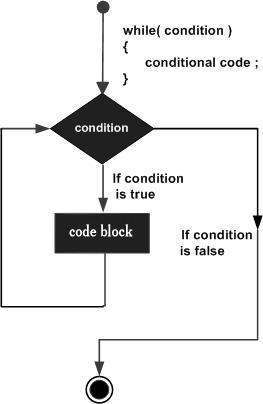
\includegraphics[width=0.4\linewidth]{P2/img/whileloop.png}
	\caption{Flow chart perulangan while}
	\label{fig:whileloop}
\end{figure}

Syntaxnya pada bahasa C adalah sebagai berikut:
% Its syntax in C programming language is as follows
\begin{verbatim}
    while(Condition)
    {
        // Blok kode yang akan diulang
    }
\end{verbatim}

Sebagai contoh, perhatikan kode berikut
% As an example, look at the following code
\begin{lstlisting}[language=c,caption = Contoh Penggunaan while,label=lst:whileexample01]
int main()
{
	int uangSaya,hargaRoti;
	uangSaya = 10000;
	hargaRoti = 2000;
	while(uangSaya >= hargaRoti)
	{
	    printf("Beli roti 1, uang saya sisa %d", uangSaya - hargaRoti);
	    uangSaya -= hargaRoti;
	}
	printf("Uang saya tidak cukup lagi");
	return 0;
}
\end{lstlisting}
Keluaran program di Listing \ref{lst:whileexample01} adalah sebagai berikut
\begin{verbatim}
    Beli roti 1, uang saya sisa 8000
    Beli roti 1, uang saya sisa 6000
    Beli roti 1, uang saya sisa 4000
    Beli roti 1, uang saya sisa 2000
    Beli roti 1, uang saya sisa 0
    Uang saya tidak cukup lagi
\end{verbatim}

Pada contoh ini, operasi pada baris 9 membuat variabel \verb|uangSaya| berkurang 2000 pada setiap pengulangan hingga akhirnya nilai \verb|uangSaya| tidak lebih dari atau sama dengan \verb|hargaRoti| lagi.
% You can see the line 9 of the code causes the variable \verb|uangSaya| to have its value substracted by 2000 for every loop until \verb|uangSaya| is no longer greater than equal to \verb|hargaRoti|. 
% The loop condition will be invalid and finaly exits the loop. Then it prints "Uang saya tidak cukup lagi", the command after the while loop statement.
Kondisi perulangan akan menjadi tidak valid dan akhirnya keluar dari perulangan. Kemudian ia mencetak "Uang saya tidak cukup lagi", perintah setelah pernyataan while loop.

\subsection{do-while loop}
do-while loop sebenarnya sama seperti while loop hanya saja do-while akan menjalankan perintah pada blok kode didalamnya sekali sebelum melakukan pengecekan kondisi.
% do-while loop is very similar to while loop. The only difference is that do-while loop will execute the code block inside it once, and then checks the condition.
\begin{figure}[H]
	\centering
	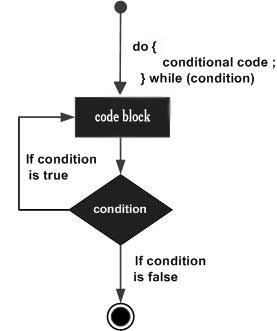
\includegraphics[width=0.4\linewidth]{P2/img/dowhileloop.png}
	\caption{Pernyataan do-while}
	\label{fig:dowhileloop}
\end{figure}
Syntaxnya pada bahasa C adalah sebagai berikut:
% Its syntax in C is as follows:
\begin{verbatim}
    do{
        // the block of code that will be repeated
    }while(Condition)
\end{verbatim}
Sebagai contoh, perhatikan kode berikut
% Look at the following example.
\begin{lstlisting}[language=c,caption = Contoh Penggunaan do-while,label=lst:dowhileexample01]
int main()
{
	int uangSaya,hargaRoti;
	uangSaya = 10000;
	hargaRoti = 12000;
	do{
	    printf("Beli roti 1, uang saya sisa %d", uangSaya - hargaRoti);
	    uangSaya -= hargaRoti;
	}while(uangSaya >= hargaRoti)
	printf("Uang saya tidak cukup lagi");
	return 0;
}
\end{lstlisting}
Output dari program pada Listing \ref{lst:dowhileexample01} adalah
% The output of the code above are
\begin{verbatim}
    Beli roti 1, uang saya sisa -2000
    Uang saya tidak cukup lagi
\end{verbatim}
% The variable \verb|uangSaya| is substracted by \verb|hargaRoti| before checking the \verb|uangSaya>=hargaRoti| condition.
% Had the code above uses while loop, the repeating block of code wouldn't have executed even once.
Variabel \verb|uangSaya| dikurangi dengan \verb|hargaRoti| sebelum memeriksa \verb|uangSaya>=hargaRoti| kondisi.
Seandainya kode di atas menggunakan perulangan while, blok kode yang berulang tidak akan dieksekusi sekali pun.
\subsection{Perulangan for}
Misalkan terdapat blok kode while dengan bentuk seperti ini:
% If you have a block of code like this:
\begin{verbatim}
    InitializationStatement; // e.g.: int i = 0;
    while(Condition){
        // do something
        updateStatement; // e.g.: i++ 
    }
\end{verbatim}
Hal ini setara dengan
\begin{verbatim}
    for(InitializationStatement;Condition;updateStatement){
        // do something
    }
\end{verbatim}

Sebagai contoh, perhatikan program berikut:
% As example, look at the following code:
\begin{lstlisting}[language=c,caption = Contoh Penggunaan for,label=lst:forexample01]
int main()
{
    int i=0;
    for(i=1;i<10;i++){
        printf("%d ",i);
    }
	return 0;
}
\end{lstlisting}
Output dari program ini adalah
% The output of this program are
\begin{verbatim}
    1 2 3 4 5 6 7 8 9 
\end{verbatim}
Berikut kode pada Listing \ref{lst:forexample01} jika diubah menjadi bentuk while-loop
% The following is the code if code in Listing \ref{lst:forexample01} converted to its while-loop form
\begin{lstlisting}[language=c,caption = For dalam bentuk while,label=lst:forwhileform01]
int main()
{
    int i=0;
    i=1;
    while(i<10){
        printf("%d ",i);
        i++;
    }
	return 0;
}
\end{lstlisting}
\begin{center}
	\colorbox{pink}{\parbox{0.8\linewidth}{\textbf{Catatan:} Terdapat keyword break dan continue yang bisa digunakan untuk mengendalikan (kontrol) alur pada perulangan. Pelajari secara mandiri!}}
\end{center}

\subsection{Tugas Pendahuluan}
\begin{enumerate}
	\item Apa yang terjadi jika kita menuliskan \verb|break;| dalam blok kode sebuah perulangan?
	\item Buatlah program dalam bahasa C yang menghitung faktorial dari sebuah bilangan bulat non-negatif yang dimasukkan oleh pengguna menggunakan loop do-while. Tampilkan hasilnya.
	\item Buatlah program dalam bahasa C untuk mencari bilangan prima antara 1 dan 100. Gunakan loop for untuk mengiterasi melalui semua angka dan pernyataan continue untuk mengabaikan angka yang bukan prima. Tampilkan semua bilangan prima yang ditemukan.
\end{enumerate}

\section{Array}
Array adalah koleksi data dimana setiap elemen mempunyai nama yang sama dan bertipe sama. Setiap elemen diakses berdasarkan  indeks elemennya.
% Array is a collection of data where each element of it has the same name(indexed) and data type. Every element in an array can be accessed using its element index.
\subsection{Array 1D}
Variabel array dimensi satu dideklarasikan dengan menentukan jenis elemen dan jumlah elemen yang di perlukan oleh array.
% One dimensional array variable can be declared by deciding the data type of the element and the number of element that is needed.

Syntax:
\begin{verbatim}
    DataType variableName [arraySize];
\end{verbatim}
\begin{enumerate}
	\item \verb*|DataType|.\\
	      % The data type of the elements in the array, e.g. \verb|float|, \verb|int|, etc.
	      Tipe data yang akan digunakan untuk array :\verb*|float|,\verb*|int|,\verb*|char| dsb
	\item \verb*|variableName|\\
	      Nama variabel mengikuti aturan pemberian nama variabel,
	      % variableName follows the variable naming convention
	\item \verb*|arraySize| \\
	      % Integer more than 0. Defining the number of element an array has.
	      konstanta integer lebih besar dari 0. \\
\end{enumerate}

Untuk menginisialisasi array dimensi satu, dapat dilakukan dengan cara seperti berikut:
% Initializing one dimensional array can be done like shown below:
\begin{verbatim}
    int contoh_array[5] = {4,2,0,6,9};
\end{verbatim}

Data di dalam array dapat akses dengan menggunakan suatu bilangan yang merupakan index dari array tersebut. Perhatikan potongan kode berikut.
% Data in an array can be accessed by using an integer that is the index of the array. Look at the code below

\begin{lstlisting}[language=c,caption = Contoh Mengakses Array 1D,label=lst:array1d01]
int main()
{
    int arr[5] = {4,2,0,6,9};
    printf("%d\n",arr[0]);
    printf("%d\n",arr[4]);
    int i = 0;
    printf("%d\n",arr[i]);
    for(i=0;i<5;i++)
        printf("%d",arr[i]);
}
\end{lstlisting}

Potongan kode pada Listing \ref{lst:array1d01} akan memberikan output
% The code in Listing \ref{lst:array1d01} will give output
\begin{verbatim}
    4
    9
    4
    42069
\end{verbatim}

\subsection{Array 2D dan Array Multidimensi lainnya}%Array 2D dan Array Multidimensi lainnya}
Array dimensi dua pada dasarnya hanya merupakan array dimensi satu di dalam array dimensi satu. Oleh karena itu, untuk mendeklarasikan array dimensi dua kita dapat menggunakan syntax seperti berikut.
% 2D array is basically a 1D array of 1D array. Intuitively, you can define a 2D array like as seen below:
\begin{verbatim}
	DataType variableName[arraySize1][arraySize2];
\end{verbatim}
Hal ini berlaku juga untuk array dengan dimensi lebih dari dua.
% This also applies to multidimensional array.
\begin{verbatim}
    DataType variableName[arraySize1]...[arraySizeN];
\end{verbatim}
Akan ada $arraySize_1\times arraySize_2 \times \cdots \times arraySize_n$ elemen yang akan dialokasikan ke memori setelah melakukan array multidimensi seperti itu
% There will be $arraySize_1\times arraySize_2 \times \cdots \times arraySize_n$ of elements that would be allocated to the memory after doing multidimensional array like that.

Untuk menginisialisasi suatu array multidimensi dapat dilakukan sama seperti array biasa:
% To initialize multidimensional array, you can do the following:
\begin{verbatim}
    int arr[2][2] = {{1,2},{3,4}};
\end{verbatim}

\subsection{Tugas Pendahuluan}
\begin{enumerate}
	\item Buatlah suatu program yang menerima input dari pengguna berupa angka 1 hingga 9, lalu memasukkan semua angka tersebut ke dalam suatu array!
	      % \item create a program to fill the data of an array by keyboard input.
	\item Apakah yang akan terjadi jika suatu array \verb|arr| diakses dengan \verb|arr[-1]|?
	      % \item What would happen if an array \verb|arr| is accessed with \verb|arr[-1]|?
	\item Apakah yang akan terjadi jika suatu array \verb|arr| dengan ukuran 5 diakses dengan \verb|arr[5]|?
	      % \item What would happen if an array \verb|arr| with size 5 is accessed with \verb|arr[5]|?
	\item Lihatlah kode berikut
	      % \item Look at the following code
	      \begin{verbatim}
        for(i=0;i<10;i++){
            for(j=i;j<10;j++){
                printf("A");
            }
        }
    \end{verbatim}
	      % How many "A" will be printed on the screen if that block of code is executed?
	      Ada berapa banyak huruf A yang akan muncul pada layar jika program tersebut dijalankan?
\end{enumerate}

\section{String}
Secara umum, string merupakan kumpulan dari satu atau lebih karakter. Spesifik pada bahasa C, string didefinisikan sebagai kumpulan karakter yang diakhiri oleh karakter null \verb|'\0'|.
\\
Misalkan string  \verb|"Dasar"|, pada bahasa C direpresentasikan sebagai kumpulan karakter \verb|'D'|, \verb|'a'|, \verb|'s'|, \verb|'a'|, \verb|'r'|, dan \verb|'\0'|.

\subsection{Penggunaan String}
Karena string tidak lain adalah array dari char, maka cara pembuatan tipe data string dalam bahasa C juga sama seperti cara pembuatan array. Berikut contohnya:
\begin{lstlisting}[language=c,caption = Contoh String dari Char,label=lst:array1d01]
	#include <stdio.h>
 
	int main(void)
	{
	char foo[8] = {'b','e','l','a','j','a','r','\0'};
	printf("Isi variabel foo adalah %s \n", foo);
	
	return 0;
	}
\end{lstlisting}

\verb|‘\0’| adalah salah satu syarat pembuatan string di dalam bahasa C.
Semua string harus memiliki karakter “khusus” untuk menandakan akhir dari string.
Tanda \verb|‘\0’| mewakili karakter null yang dipakai oleh compiler bahasa C sebagai tanda akhir sebuah string.

Contoh source code penggunaan \verb|scanf| untuk membaca string:
\begin{lstlisting}[language=c,caption = Contoh String dengan scanf,label=lst:scanf]
	#include <stdio.h>

	int main() {
		// Mendeklarasikan variabel untuk menyimpan input dari pengguna
		int age;
		float height;
		char name[50];

		// Meminta pengguna untuk memasukkan usia mereka
		printf("Masukkan usia Anda: ");
		scanf("%d", &age);
		
		// Meminta pengguna untuk memasukkan tinggi mereka
		printf("Masukkan tinggi Anda (dalam meter): ");
		scanf("%f", &height);
		
		// Meminta pengguna untuk memasukkan nama mereka
		printf("Masukkan nama Anda: ");
		scanf("%s", name);

		// Menampilkan informasi yang dimasukkan pengguna
		printf("Nama: %s\n", name);
		printf("Usia: %d tahun\n", age);
		printf("Tinggi: %.2f meter\n", height);

		return 0;
	}
\end{lstlisting}


Contoh source code penggunaan \verb|gets| untuk membaca string:
\begin{lstlisting}[language=c,caption = Contoh String dengan gets,label=lst:gets]
#include <stdio.h>

int main () {
  
	char arr[100];
	while(true)
	{
		gets(arr);
		
		printf("-- %s\n", arr);
	}
  return 0;

}
\end{lstlisting}

String yang dibaca dengan mengunakan scanf atau gets akan secara otomatis memiliki \verb|null| character di akhir.

\subsection{Fungsi-Fungsi String}
Dalam bahasa pemrograman C, terdapat library yang dibuat dengan tujuan memudahkan pengguna dalam mengolah string.
Library tersebut tersimpan dalam \verb|<string.h>|,
oleh karena itu, untuk mengakses library ini, diperlukan tambahan preprocessor, yaitu:
\begin{lstlisting}[language=c]
	#include <string.h>
\end{lstlisting}

Pelajari berbagai fungsinya di \href{http://www.cplusplus.com/}{www.cplusplus.com}.

\subsection{Tugas Pendahuluan}
\begin{enumerate}
	\item Buatlah program dalam bahasa C yang mengambil dua string dari pengguna dan menentukan apakah kedua string tersebut anagram (mengandung karakter yang sama dalam urutan yang berbeda).
		  Misalnya kata "usap" dan "sapu".
	      Tampilkan pesan yang sesuai.
	\item Sebutkan 5 fungsi yang terdapat pada library \verb|string.h|! jelaskan kegunaan masing-masing fungsi tersebut!
	\item Untuk mengeluarkan output string, selain menggunakan \verb|printf()| kita juga bisa menggunakan \verb|puts()|. Jelaskan kelebihan menggunakan \verb|puts()| jika dibandingkan dengan \verb|printf()|!
\end{enumerate}